 \documentclass[12pt,relax]{article}
 \usepackage{graphicx}
% DisplayCommand
\newcommand{\DisplayCommand}[1]{%
  \par\vspace{1ex}%
  {\bf Command:}%
  {\hspace{0.2 in}} {\tt #1} {\par\vspace{1ex}}}

% InlineCommand
\newcommand{\InlineCommand}[1]{
  {\hspace{0.01 in}} {\tt #1} {\hspace{0.01 in}}}

% InlineDirectory
\newcommand{\InlineDirectory}[1]{
  {\hspace{0.01 in}} {\tt #1} {\hspace{0.01 in}}}

\usepackage{array}
    \title{An Introduction to Eight Valuable Software Quality Tools}

\author{
James M. Willenbring \\
 \\
St. Cloud State University\\
Computer Science Department\\
CS 680 Term Paper
}

    % There is a "Printed" date on the title page of a SAND report, so
    % the generic \date should generally be empty.
    \date{December 19, 2003} % Remove ``\today'' in final version



\author{
James M. Willenbring \\
Computational Math and Algorithms Department \\
 \\
Sandia National Laboratories \\
P.O. Box 5800 \\
Albuquerque, NM 87185-1110}

\begin{document}
\maketitle
%\setcounter{page}{3} % Accounts for blank page at beginning
%\begin{abstract}

%**Fill in Abstract

%\end{abstract}

\clearpage

\section*{Acknowledgments}

The author would like to acknowledge the support of the ASCI and LDRD 
programs that funded development of Trilinos and recognize all Trilinos 
contributors: Michael Heroux (project leader), Teri Barth, Ross Bartlett, 
David Day, Robert Heaphy, Robert Hoekstra, 
Jonathan Hu, Tammy Kolda, Richard Lehoucq, Kevin Long, Eric Phipps, 
Roger Pawlowski, Andrew Rothfuss, Andrew Salinger, Paul Sery, Ken
Stanley, Heidi Thornquist, Ray Tuminaro and Alan Williams.

In particular, Tammy Kolda deserves thanks for suggesting the topic for
this paper.  Also, Michael Heroux deserves credit for designing 
reasonable typographical conventions and for providing comments on the draft
versions of the paper.

\clearpage
\tableofcontents
\listoffigures
\listoftables

\clearpage
%The following file is also used in the User Guide
%\begin{itemize}
\item[Trilinos]
The name of the project.  Also a Greek term which,
loosely translated means ``a string of pearls,'' 
meant to evoke an image that each Trilinos package is a pearl in its 
own right, but is even more valuable when combined with other 
packages.

\item[Package]
A self-contained collection of software in Trilinos
focused on one primary class of numerical
methods.  Also a fundamental, integral unit in the Trilinos framework.

\item[new\_package] A sample Trilinos package containing all of the
infrastructure to install a new package into the Trilinos framework.
Contains the basic directory structure, a collection of sample
configuration and build files and a sample ``Hello World'' package.
Also a website.

\item[Anasazi]
An extensible and interoperable framework for large-scale eigenvalue
algorithms.The motivation for this framework is to provide a generic
interface to a collection of algorithms for solving large-scale 
eigenvalue problems.

\item[AztecOO] 
Linear solver package based on preconditioned Krylov methods.  A 
follow-on to the Aztec solver package~\cite{Aztec2.1}.  
Supports all Aztec 
interfaces and functionality, but also provides significant new 
functionality.

\item[Belos] A Greek term meaning ``arrow.'' Belos is the next
generation of iterative solvers.  Belos solvers are written using
``generic'' programming techniques.  In other words, Belos is written
using TSF abstract interfaces and therefore has no explicit dependence
on any concrete linear algebra library.  Instead, Belos solvers can be
used with any concrete linear algebra library that implements the TSF
abstract interfaces. 

\item[Ifpack] 
Object-oriented algebraic preconditioner, compatible with 
Epetra and AztecOO.  Supports construction and use of parallel
distributed memory preconditioners such as overlapping Schwarz domain
decomposition, Jacobi scaling and local Gauss-Seidel relaxations.

\item[Komplex] 
Complex linear equation solver using equivalent real 
formulations~\cite{DayHero2000}, built on top of Epetra and AztecOO.

\item[LOCA]
Library of continuation algorithms. A package of scalable stability 
analysis algorithms (available as part of 
the NOX nonlinear solver package). When integrated into an application code, 
LOCA enables the tracking of solution branches as a function of system 
parameters and the direct tracking of bifurcation points.

\item[Meros]
Segregated preconditioning package.  Provides scalable block
preconditioning for problems that couple simultaneous solution
variables such as Navier-Stokes problems. 

\item[ML]
Algebraic multi-level preconditioner package.  Provides scalable
preconditioning capabilities for a variety of problem classes.  

\item[NOX]
A collection of nonlinear solvers, designed to be easily integrated
into an application and used with many different linear solvers.

\item[Petra]
A Greek term meaning ``foundation.''  Trilinos has three Petra 
libraries: Epetra, Tpetra and Jpetra that provide basic classes 
for constructing and manipulating matrix, graph and vector
objects.  Epetra is the current production version that is
split into two packages, one core and one extensions.

\begin{itemize}

\item[Epetra] Current C++ production implementation of the Petra
Object Model.  The ``E'' in Epetra stands for ``essential'' implying
that this version provides the most important capabilities that are
commonly needed by our target application base.  Epetra supports real,
double-precision floating point data only (no single-precision or
complex).  Epetra avoids explicit use of some of the more
advanced features of C++, including templates and the Standard
Template Library, that can be impediments to portability.

\item[Tpetra] The future C++ version of Petra, using templates and
other more advanced features of C++.  Tpetra supports arbitrary scalar
and ordinal types, and makes extensive use of advanced C++ features.

\item[Jpetra] A Java implementation of Petra, supporting real,
double-precision data.  Written in pure Java, it is designed to be
byte-code portable and can be executed across multiple compute nodes.

\end{itemize}

\item[Teuchos] A collection of classes and service software that is
useful to almost almost all Trilinos packages.  Includes
reference-counted pointers, parameter lists, templated interfaces to
BLAS, LAPACK and traits for templates.  

\item[TSF] A collection of abstract interfaces that supports application
access to a variety of Trilinos capabilities, supports
interoperability betweeen Trilinos packages and provides future extensibility.
TSF is composed of several packages.  The primary user packages are:  
\begin{itemize}

\item[TSFCore] TSFCore provides 
a basic collection of abstract interfaces to vectors, linear
operators, solvers, etc.  These interfaces provide a common
interface for applications to access one or more packages that
implement the abstract interface.  These interfaces can also be used
by other packages in Trilinos to accomplish the same purpose.

\item[TSFExtended] TSFExtended builds on top of TSFCore, providing implicit
aggregation capabilities and overloaded operators.  
\end{itemize}
\end{itemize}


%Nomenclature
%** Fill in

\section{Introduction}
\label{Section:Introduction}

Many software developers cringe at the very words ``Software Quality 
Assurance''.  Thoughts of practices that will marginally improve software 
quality while primarily functioning as a huge time sink come to mind.  This 
fear is not entirely unfounded.  Many software quality practices do take a lot 
of time without providing measurable improvements in quality.

Almost two years ago the Trilinos development team was charged with the task 
of improving existing software quality practices.  The goal was to implement 
software quality tools that improve both software quality and developer 
productivity.  This paper will introduce eight of the tools that were 
chosen by the Trilinos development team.

Readers do not need a thorough understanding of the Trilinos project.  
Important characteristics about the Trilinos project will be presented 
as necessary.  The tools discussed are presented because they are generally 
useful for software projects.

Those who are interested in learning more about the Trilinos project should 
consult {\it An Overview of Trilinos}~\cite{Trilinos-Overview} or the
{\it Trilinos Users Guide}~\cite{Trilinos-Users-Guide}.  Trilinos also has an 
excellent web site that can be found at 
\InlineDirectory{http://software.sandia.gov/trilinos}~\cite{Trilinos-home-page}.

Before discussing the individual tools, we will introduce three categories of 
people who are involved in software development in different ways and 
as a result
will utilize the various tools in different ways.
\subsection{Typographical Conventions}

Typographical conventions used in the paper are found in
Table~\ref{Table:TypoConventions}.
\begin{table}[ht]
\scriptsize
\begin{center}
\begin{tabular}{|l|l|p{2.0in}|} \hline
Notation & Example & Description \\ \hline
\InlineCommand{Verbatim text} & \InlineCommand{../configure --enable-mpi} & 
URL's, commands, directory and file name examples, and other text associated
with text displayed in a computer terminal window. \\ \hline
\InlineCommand{CAPITALIZED\_TEXT} & \InlineCommand{CXXFLAGS} & 
Environment variables used to configure how tools such as compilers behave. \\ \hline
\InlineCommand{<text in angle brackets>} & \InlineCommand{../configure
<user parameters>} & 
Optional parameters. \\ \hline
\end{tabular}
\end{center}
\caption{\label{Table:TypoConventions} Typographical Conventions for This Document.}

\end{table}

\section{Players in the Software Development Process}
%Try to change this lousy title
Those involved in the software development process can be separated into 
several different categories.  For the purposes of this paper, three 
categories of ``players'' with be considered: developers, users (including 
system administrators and end users), and management.  The developer and user 
categories are self-explanatory.  The management category includes the those 
who must keep up with what is going on in the project to various degrees, but 
do not necessarily fall into the user or developer category.  Examples include 
the managers of both users and developers and those affiliated with a funding 
source for the project.  There may be situations in which an individual fits 
into more than one category.

The members of the three categories have different functions in the 
development process and will find the various tools to be useful 
in different ways.  Some players will have no use at all for certain tools.
Throughout the paper, the ways in which the various categories of players 
can best utilize the individual tools will be discussed.  Which features any 
given individual might wish to use obviously will vary.

\section{A Description of the Software Quality Tools}
\label{Section:CommunicationTools}

This section will introduce the tools that the Trilinos team has implemented 
which have improved the quality of the Trilinos software and increased the 
productivity of the team.  The tools discussed are CVS, Bugzilla, Mailman, 
Bonsai, Doxygen, GNU Autoconf and Automake, and COVTOOL.

While reading about the various tools in the rest of this section, pay 
particular attention to how some of the tools can interact with one another.
For example, CVS commit messages are broadcast using a Mailman mail list.
The value of adopting a set of useful software quality tools extends far 
beyond the sum of the value of the individual tools.

Also, many development teams uphold a level of software quality that is far 
higher than the level that the team can prove is maintained.  If comprehensive
regression tests are run, design specifications are approved by the 
proper individuals, and issue reports are addressed in a timely manner, but 
there is no record that any of this happened, it doesn't mean much to an 
auditor or a funding source.  Notice how many of these tools are virtually
self-documenting.  The tools themselves are generally easy to use, and 
record artifacts at no additional effort on the part of a developer.  

%Bugzilla is an 
%issue tracking tool.  Mailman provides the ability to set up mail lists and 
%archives all messages sent to the lists.  

\subsection{CVS Repository}

One of the first steps that should be taken to improve software quality is the 
adoption of a version control system.  Trilinos source code is maintained in a 
Concurrent Versions System~\cite{CVS}
(CVS) repository.  It is very easy to add new files and directories to
the repository.  Projects that already use CVS and are to be merged with 
another project can even retain their CVS history!

A CVS repository stores all of the information about current and past versions
of all of the files in a project.  (To provide for a safe backup of the 
project, the CVS repository itself should be backed up on a regular basis.)  
Developers can ``checkout'' a snapshot of 
the repository, edit one or more files and then ``commit'' the changes to the
repository.  Complicated situations arise when multiple developers are 
editing the same files at the same time.  How these potential ``conflicts'' 
are resolved is beyond the scope of this document.  Suffice it to say that 
CVS handles all of the situations that it can.  When it cannot safely handle 
the situation, it provides a developer with a clear description of which 
lines of code are in conflict so that the developer can resolve the 
conflict more quickly.  The ability to checkout a snapshot of the 
repository from the past has many obvious advantages including making it easy 
to revert back to an old version of a piece of code that is found to be not 
portable to an important platform and making it possible to pinpoint the exact 
commit that caused an error.

Some of the most useful features of CVS include the fact that a CVS 
repository can be set up in such a way that it is accessible from anywhere, 
and the ability to create multiple ``branches'' of the same project.  For 
example, a development branch and multiple release branches would be 
appropriate for most software projects.  Patches that are applied 
to a release branch can be ``merged'' back into the development branch.  
In addition, security can be enforced in a fine-grained manner if necessary.  

One aspect of using CVS that deserves to be stressed is that comments can be 
made with each commit.  The Trilinos team has found that these comments are 
very important.  A well thought out comment is very helpful when trying to 
debug at a later time.  Even if a commit doesn't make any major changes to the 
code, it is useful to briefly describe what was done.  Some changes that may 
seem to be minor might not be portable.  At the very least, a comment could 
help a developer to rule out a particular commit as the inception point 
of a bug.

Another endearing feature of CVS is that other software quality tools can 
interact seamlessly with CVS.  For example, CVS commit messages can be sent to
a Mailman mail list for distribution.  Also, Bonsai provides a convenient 
interface for accessing CVS information.  See section~\ref{subsect:Bonsai} 
for a thorough description about how the details of CVS commits are accessible 
via Bonsai.

The primary beneficiaries of the capabilities of CVS are the project 
developers.  The developers are the ones who will be interested in merging 
changes, resolving conflicts, creating release branches, and using the more 
advanced features of CVS.  In some cases, it makes sense to give 
important users direct access to the CVS repository.  With direct access, 
users are able to receive patches and new release versions as soon as they 
become available.  Users who are on the ``bleeding edge'' of a project will 
probably want CVS access.

CVS is a great tool, one that might be considered to be ``smart''.  Some 
Trilinos developers were a little wary about whether or not CVS would be able
resolve conflicts properly in all cases.  After nearly two years, the author is
not aware of any instances where CVS has improperly merged two changes.  If in 
doubt, CVS leaves the merging process to the developer.

CVS has many more features than those that were described above.  For a more 
complete listing of CVS features and a description of valid CVS commands, 
see the GNU CVS Home Page~\cite{CVS}.  Those who still want more information 
might wish to obtain a copy of 
{\it Open Source Development with CVS}~\cite{CVSbook}.

\subsection{Bugzilla}
\label{subsect:Bugzilla}
An important step in achieving a high level of software quality is tracking
and organizing issues pertaining to faults in the software and issues related 
to enhancement requests.  The Trilinos team has implemented a tool called 
Bugzilla~\cite{Bugzilla} to achieve this end.  Bugzilla  can be found 
on the web at \InlineDirectory{http://www.bugzilla.org}.

All issues related to any Trilinos package are submitted to Bugzilla.  This 
even applies to cases in which 
one developer diagnoses and fixes a bug within a short period of time.  A bug 
report is still very valuable in this case because it provides an artifact 
that outlines the problem and explains how the problem was fixed.  A bug 
report should be filled out with as much detail as possible.  Likewise, after 
a bug has been resolved, the developer should also provide a detailed 
description of the solution that was used.  These detailed descriptions have 
been used to quickly diagnose problems that tend to come up again and again.
For example, if a particular supported platform doesn't have a header file 
that is widely considered to be ``standard'', multiple developers might try 
to use a similar piece of code that is not portable.  A detailed bug report 
will easily be found based on key words or another piece of relevent search 
criteria, and will also provide a description of the problem and quite 
possibly an alternative technique that will fix the issue. 

Issues tracked by Bugzilla can be searched by owner, platform, and many other 
criteria.  Figure(***) shows the Bugzilla search screen for Trilinos.  The 
interface for entering and searching for bugs is both user friendly and 
customizable.  Major pieces of a software project can be 
designated as ``products'', different aspects of those products can be 
listed as ``components'', and versions of the various products can also be 
entered.  This breakdown makes it easy to categorize and find issues in the 
Bugzilla database.  For example, Trilinos is composed of individual 
``packages''.  Each package has been designated as a Trilinos product.  One of 
the packages within Trilinos is called Epetra.  So a user who is searching for 
a fix for a build error while building Epetra on a particular 
machine should select ``Epetra'' in the product field, ``Configuration and 
Building'' in the component field, select the applicable hardware and OS, and
could also fill in the version field.  Issues can be assigned to any 
individual with a Bugzilla account.  If a 
person who is entering a bug report does not know who to assign the bug to,
the bug can be assigned to a default owner of the selected component 
by leaving the ``Assigned To'' field blank.  

%\begin{figure}
%\begin{center}
%\includegraphics[height=6in,angle=90]{Bugziila-enter.gif}
%\end{center}
%\caption{\label{Figure:TrilinosPackages}Current collection of Trilinos Packages}
%\end{figure}

When submitting an issue, a 
priority and severity of the bug can be selected (and later changed by the 
issue owner if desired).  Priority and severity are related, but certainly are 
not the same.  Priority refers to the order in which the issue should be 
resolved relative to other issues.  Severity refers to what degree the issue 
negatively affects the proper functions of the software.  Often there is a 
correlation between priority and severity; however, this does not have to be
the case.  For example, an issue that reports a build failure on a 
machine should be given a severity of ``blocker'' (the highest level of 
severity), but might be given a low priority because the build failure occurs
on a platform that is not supported.  Conversely an ``enhancement'' (the 
lowest severity level) might be a very high priority issue.  Regardless of the 
priority and severity assigned to an issue, the issue will not be forgotten 
about in the way that issues sometimes simply fall through the cracks if not 
properly recorded~\cite{Bugzilla}.

In addition to the basic functionality described above, Bugzilla provides some 
useful advanced features.  The more advanced features include
granular security checking, the ability to integrate information with 
other software development tools including CVS, and inter-bug 
dependencies and dependency tracking~\cite{Bugzilla}.  Dependency tracking 
makes it easy to see the relationship 
between bugs.  The Trilinos team has introduced the concept of a metabug which 
is a larger task that is dependent on multiple smaller tasks.  Each of the 
smaller tasks can be assigned to different people. Metabugs make it is easy 
for project leaders (or management) to track the status of important issues. 

Bugzilla is an extremely useful tool for developers, users and management.  
Developers will especially appreciate the ability to search for issues 
that have been assigned to them and the database of knowledge that grows over
time.  The Trilinos bugzilla database contains over six hundred issues and 
has served as a quick reference to numerous problems that took hours, days 
or even weeks to solve the first time that the issue was encountered.  The 
Bugzilla interface has led to a noticeable increase in the quality of 
issue submissions.  By providing fields that can be filled in, those who are 
submitting issues tend to provide more information than they would when just 
sending an email to a developer about a problem.  This results in quicker 
issue resolution and a better record of the issue after it has been resolved.  

Users frequently take advantage of Bugzilla's search capability to check on 
the status of issues that they have submitted.  Users also benefit from the 
easy to use interface for submitting issues and from the ability to submit 
issues to default component owners.  

Bugzilla provides management with a quick snapshot of the status of the 
project.  It can also provide more detailed information about pressing issues.

NOTE: In the context of Bugzilla, ``bug'' and ``issue'' are generally 
interchangeable and can refer not only to an error in 
existing code, but also to a desired enhancement.  For example, a bug report 
should be submitted to Bugzilla to report a segmentation fault, and a bug 
report should also be submitted to request a new feature.

\subsection{Mailman}
\label{subsect:MailMan}
Mailman~\cite{Mailman} is a relatively simple tool that helps facilitate 
communication between
those involved with a project and helps to extend the usefulness of other 
software development tools.  It can be found on the web at 
\InlineDirectory{http://www.list.org}.  Mailman can be used to establish any 
number of 
email lists for a project.  It is advantageous to set up email lists because exactly 
those people who have declared themselves to be interested in a 
topic can be included in the circulation of the discussion.  Without 
mail lists, those who might have insight into an issue can easily be forgotten 
when sending an email.  Conversely, if people routinely get a lot of emails 
concerning topics that they do not care about, some will begin deleting
their email without reading through it.  

A specific example of how Mailman 
has had a positive impact on the Trilinos project is that when a new person
joins the development team or becomes a user, that person is able to 
subscribe to the appropriate mail lists and is instantly involved in the 
conversations that take place.  The mail list archives are also searchable, 
which allows people new to Trilinos to catch up on interesting events from the 
past.  Obviously, the searchable archives are useful for new and existing 
developers, users and management.  The self-documenting feature provided 
by Mailman's searchable archives is also useful for audits.  It provides a 
``paper trail'' for major decisions that were arrived at and closely follows 
the evolution of the entire project, especially when Mailman is used in 
conjunction with other tools such as CVS.

One advanced feature of Mailman that is worth noting is the digest mode option.
This option gathers all of the emails sent to a particular list for an entire 
day and sends them out together in one email.  For those who are not closely 
involved with the discussions that take place on particular lists but want to 
keep up with what is happening in general, digest mode can be a very 
attractive option.  For extremely urgent messages, digest mode can 
be overridden.

The Trilinos project maintains more than ninety separate mail lists through 
Mailman.  Mail lists are maintained for Trilinos as a whole and for each 
package.  A partial list of the current Trilinos mail lists can be seen in 
Figure~\ref{Figure:mailman}.  
Additional mail lists can be set up very easily.  Each Trilinos 
package usually has five mailing lists.  The example mailing lists mentioned 
below are to be used for issues relating to all of Trilinos.  
The names for the lists pertaining to individual packages follow the same 
naming scheme, simply replace ``Trilinos'' with the name of the package.  For example, the list for Trilinos users is 
called Trilinos-Users and the email address is 
\InlineCommand{trilinos-users@software.sandia.gov}  The list 
for Epetra users is called Epetra-Users and the associated email address is 
\InlineCommand{epetra-users@software.sandia.gov}.  Following a standard naming
scheme allows the name of the lists to be remembered easily.  Although the 
set of mail lists that a software project uses is fully customizable, the 
Trilinos team has found the following break down of lists to be very effective 
and would recommend the break down to other projects.

\clearpage
\begin{figure}
\begin{center}
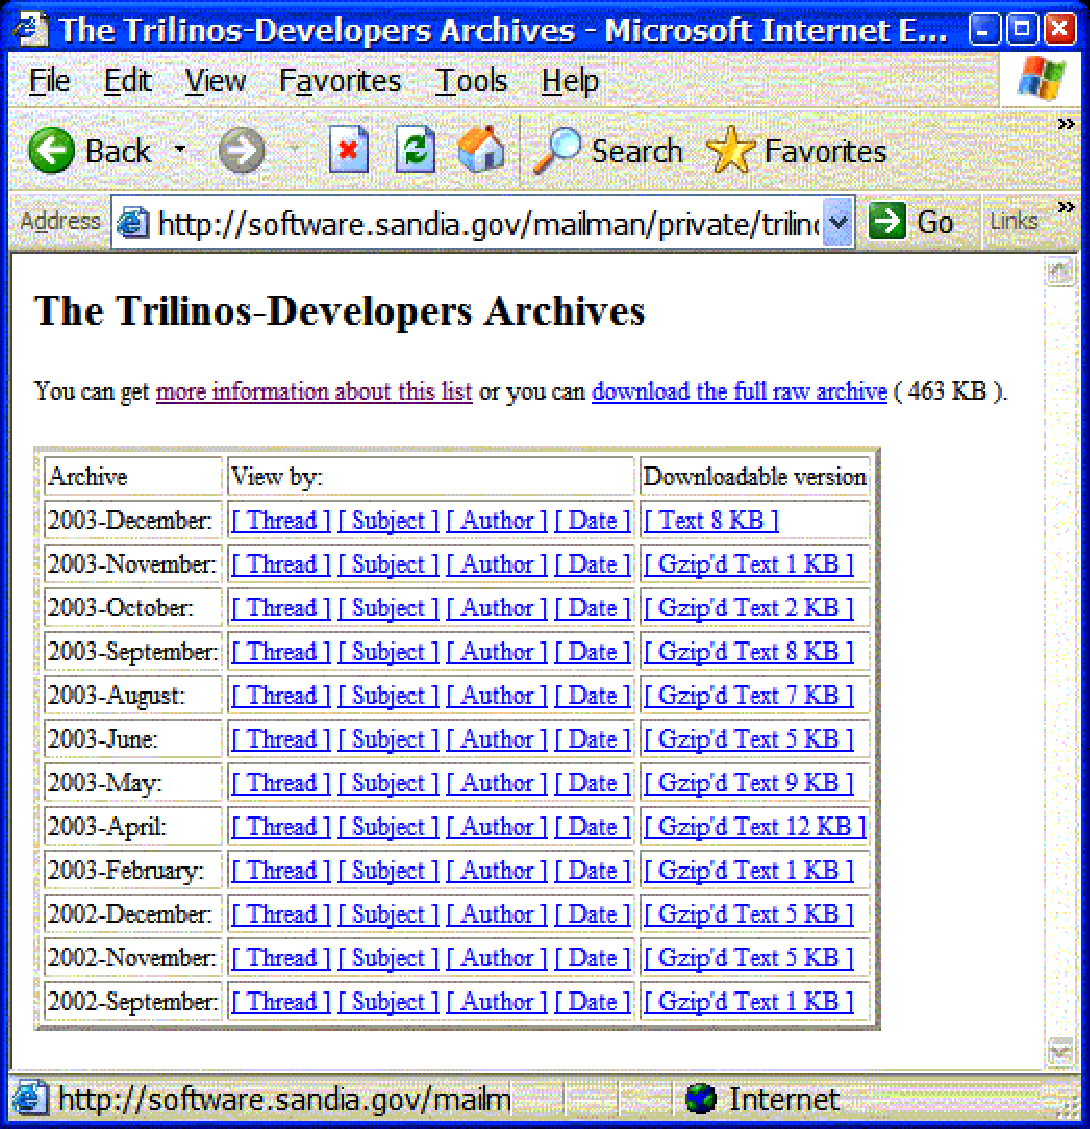
\includegraphics[scale=0.1,angle=90]{mailman}
\end{center}
\caption{\label{Figure:mailman}A partial listing of the Trilinos mail lists}
\end{figure}
\clearpage

\framebox{\begin{minipage}[r]{.75\textwidth}{
{\bf Note:}
While those who use Epetra (or any other Trilinos package) are also
``Trilinos users'', the lists are not set up to recognize this.  In other 
words, those who subscribe to the Epetra-Users mailing list do not necessarily 
form a subset of those who subscribe to the Trilinos-Users mailing list.  This 
is also true of all other list types.  
}\end{minipage}}

\begin{itemize}
\item Trilinos-Announce 
\InlineCommand{trilinos-announce@software.sandia.gov}

All Trilinos release announcements and other major news.  The appropriate 
audience for this list includes developers, users and management.

\item Trilinos-Checkins 
\InlineCommand{trilinos-checkins@software.sandia.gov}

CVS commit log messages that are related to Trilinos in general or packages 
that have not had separate lists established.  The appropriate audience for 
this list includes developers who are very closely involved with particular 
aspects of Trilinos development.  Those who are not as closely involved might 
choose to search the archives as necessary, rather than elect to receive 
each of the CVS commit log messages.

\item Trilinos-Developers 
\InlineCommand{trilinos-developers@software.sandia.gov}

All discussions related to Trilinos-specific development (not specific to a 
Trilinos package) are conducted via this list.  Important development 
decisions that originate in other places (regular email, discussions, etc) 
should also be posted to this list (or to the appropriate package list).  
By doing this, the list archive can provide records that explain why various 
changes were made over time.  As the name implies, the appropriate audience for
this list includes Trilinos developers.

\item Trilinos-regression 
\InlineCommand{trilinos-regression@software.sandia.gov}

All regression test output that is not specific to a package.  The appropriate 
audience for this list includes developers who are interested in the daily 
results of the Trilinos test harness.  In reality, few subscribe to this list.
When problems need to be tracked, the archive can provide all available 
information.  This list gathers the artifacts necessary to prove that 
regression testing takes place on a regular basis.

\item Trilinos-Users 
\InlineCommand{trilinos-users@software.sandia.gov}

List for Trilinos Users.  General discussions about the use of Trilinos.  In 
addition to users, developers also subscribe to this lists to answer user 
questions.

\item Trilinos-Leaders
\InlineCommand{trilinos-leaders@software.sandia.gov}

Mailing list for representatives for each Trilinos package.  There are no 
leaders lists for individual packages.  In addition to package leaders and 
interested developers, management will also want to subscribe to this list.
\end{itemize}

Managing the lists requires a minimal amount of overhead.  List administrators
are assigned to each list.  The administrators handle issues such as accepting
or rejecting requests for list membership and posting requests from 
non-members.  This overhead is covered many times by the fine-grained control
of information dispersal that Mailman provides and the archives that 
Mailman maintains.

\subsection{Bonsai}
\label{subsect:Bonsai}

The CVS history of a project can be made accessible via a
web-based interface program called Bonsai~\cite{Bonsai}.  This tool can be 
found on the web at 
\newline
\InlineDirectory{http://www.mozilla.org/bonsai.html}.  

\begin{minipage}[c]{\textwidth}

\begin{minipage}[l]{.6\textwidth}

Bonsai gives developers the ability to view the changes made to the files in 
the repository. Developers can search 
based on filename, directory, branch, date, user who made the 
change, or any combination of these criteria.  The differences between any two 
versions of a file may also be viewed, which can be very helpful when 
debugging.  
\end{minipage}\hfill
\framebox{\begin{minipage}[r]{.35\textwidth}{
{\bf Key Point:}
The differences between any two versions of a file may also be viewed, 
which can be very helpful when debugging.  
}\end{minipage}}
\end{minipage}

Along with the results of a search, the CVS commit messages corresponding to 
the changes that match the query are also shown.  If any Bugzilla bug numbers 
were referenced in a commit message, the number of each bug is clickable.  
Clicking on a bug number will bring up the bug in question.  

Bonsai is a tool that will almost exclusively be used by developers.  It has 
taken a long time for Bonsai to catch on with some members of the Trilinos 
development team.  This might be explained by the fact that Bonsai doesn't 
provide any capabilities that are not available via another method.  
Rather, Bonsai makes doing difficult things a lot easier.
For example, having the CVS commit message one click away from the line 
by line changes that
were made to a file can save a lot of time.  Also the file differences are 
presented in such a way that multiple lines before and after the differing 
lines are shown to provide some context for the code that was modified.  
The interface for Bonsai is very intuitive and can be learned in a matter of 
minutes.  The time spent learning how to use Bonsai will be more than made up 
for by using it to track and correct one bug.

\subsection{Doxygen}

Doxygen~\cite{Doxygen} is a tool that can be used to create 
extensive documentation for a project with little effort beyond that which is 
required to write well commented code.  The information below is limited 
to an overview of the features of Doxygen.  For information about how to use 
Doxygen, see the Doxygen 
web site at \InlineDirectory{http://www.doxygen.org}.  

Doxygen is meant to be used with C++, C, Java, and IDL, but can also be used 
in a more limited fashion to create documentation for code written in other
programming languages.  Doxygen documentation 
can be generated in several formats including HTML, LaTeX, RTF, PostScript, and
Unix man pages.  One of the most impressive features of Doxygen is its ability 
to generate dependency graphs, inheritance diagrams, and collaboration 
diagrams~\cite{Doxygen}.  For an example of a Doxygen generated inheritance 
diagram, see Figure(***).  Another impressive feature of Doxygen is that the 
documentation is very easy to navigate.  For a sample of how easily Doxygen 
documentation can be navigated go to
\newline
\InlineDirectory{http://software.sandia.gov/trilinos/packages/epetra}.  Then
click on \InlineDirectory{Documentation}, and then 
\InlineDirectory{Development Docs}. 
Throughout the documentation, the name of objects, 
the name of files, and line numbers within files are all clickable.

In a very short time, it is possible to take a well-commented piece of code 
and create nicely styled and easy to navigate documentation using Doxygen.
Developers are typically the only people who use Doxygen directly.  The 
documentation that is generated by Doxygen is obviously useful to both 
developers and users.

\subsection{Configuration Management - Autoconf and Automake}

Achieving a high level of software quality is complicated immensely when 
a software project is required to be portable to a wide array of platforms.
In the past, the Trilinos development team attempted to maintain a large 
number of platform specific makefiles to improve portability.  For the past 
year and a half, we have instead utilized GNU Autoconf~\cite{Autoconf} and 
Automake~\cite{Automake} for 
the purposes of configuring and building Trilinos, respectively.  Again, 
the below discussion will be limited to some highlighted features of Autoconf 
and Automake.  
For a complete description how to use Autoconf and Automake, see 
{\it GNU Autoconf, Automake, and Libtool}~\cite{GoatBook}, which is 
more commonly referred to as the ``Goat Book''.  (Libtool is the third tool 
in the set of three tools commonly referred to as the ``Autotools''.  Trilinos 
does not yet use Libtool, although we plan to incorporate it into the build 
process in the future.)

Unfortunately, Autoconf and Automake have not eliminated all portability 
problems for Trilinos.  We still have to provide a set platform specific
``invoke-configure''scripts to feed to Autoconf.  In addition, the learning 
curve for Autoconf and Automake was quite steep.  Despite these facts, 
as a whole, the migration to Autoconf and Automake has been quite 
beneficial.  

Autoconf provides a macro called F77\_FUNC that can be 
automatically defined during the configure stage to the proper Fortran
name mangling scheme for the platform the the configure script is run on.  
Knowing the Fortran name mangling scheme is necessary when calling routines 
from Fortran libraries such as the BLAS~\cite{BLAS1,BLAS2,BLAS3} and 
LAPACK~\cite{lapack} from a C or C++ library.  Aside from a few special cases, 
Autoconf is able to detect the proper name mangling scheme automatically.  
This eliminates the need for Trilinos packages to have ifdef's for every 
platform that doesn't use the most common scheme.

In addition, Autoconf detects which header files are present on a particular 
machine.  For example, if \InlineDirectory{cmath} is present on a machine, 
pound include that, otherwise, if \InlineDirectory{math.h} is present, pound 
include that.  If neither are present, exit configure with an error indicating 
that one of the two files is required.  Providing the appropriate ifdef's 
for header files on a per machine basis was a difficult task before the 
public release of Trilinos.  Now with users spread around the world, that 
task would be nearly impossible.  In a perfect world, every machine would 
have all of the latest standard header files available, in practice, that 
is far from the case.

Autoconf conducts many other configure time tests to determine various 
characteristics of the machine it is running on.  Additional tests can 
easily be written to test for other characteristics.  The results of these 
tests can then be used for various purposes, such as conditionally compiling 
a piece of code, or to define any number of macros.

Automake has greatly simplified the process of writing makefiles.  All a 
developer has to do is provide a few simple pieces of information, and 
Automake will generate another file called Makefile.in which is used to 
generate the appropriate Makefile during the configure stage.

As mentioned above, the learning curve for Autoconf and Automake was quite 
steep.  Fortunately, a couple of Trilinos developers have created a package 
called ``new\_package'' to jump start an effort to set up a configure and 
build system that uses Autoconf and Automake.  The effort was focused 
primarily on helping new packages join Trilinos, but directions that 
new\_package provides can be applied to more general cases as well.  Several
developers have used new\_package as a starting point for putting an additional
package into Trilinos.  It is possible to download new\_package from the 
Trilinos web site.  The specific link is 
\InlineDirectory{http://software.sandia.gov/trilinos/downloads.html}.  After
downloading new\_package, direct your attention to the README file.

Included with new\_package is a large set of M4~\cite{M4} macros that can 
be freely used by other projects.  These macros perform many common 
configuration tasks such as locating a valid LAPACK~\cite{lapack} library, 
or checking for additional values to prepend to CXXFLAGS that have been 
specified by a user.  The macros can be found in the \InlineDirectory{config}
subdirectory of the new\_package download.  These macros minimize the amount of
redundant effort in using Autoconf and make easier to apply a common change to 
multiple projects.  The M4 macros are meant to supplement the large number of 
macros that come with Autoconf.  Additional M4 macros that are designed for 
specialized tasks are also available at various sites on the web.

Developers and users will both make use of Autoconf and Automake.  Developers 
obviously need to set up the system, but users also need to know at least a 
little bit about Autoconf and Automake.  Minimally, users need to call the 
configure script with any appropriate arguments.  Sometimes users end up 
learning quite a bit about how Autoconf and Automake work because, as stated 
earlier, Autoconf and Automake do not make portability a trivial issue.  It is 
doubtful that any tool will ever make porting a trivial issue.  However, a 
configure and build system using Autoconf and Automake is a 
noticeable improvement over a more traditional system using simple makefiles.

\subsection{COVTOOL}

A very important part of Software Quality Assurance is incorporating 
comprehensive regression testing.  The effectiveness of regression tests is 
difficult to measure.  One measure that is used is code coverage percentage.  
The code coverage percentage of a regression test suite can be calculated by 
dividing the number of lines of code that are executed when running the 
regression test suite by the total number of lines of code in the project.
A high code coverage percentage does not guarantee that a regression test 
suite is effectively testing the code, but a low code coverage percentage does 
guarantee that the regression test suite is not effective.

Some Trilinos development team members have begun to use a code coverage tool 
called COVTOOL~\cite{COVTOOL} to calculate code coverage percentages for 
Trilinos packages.  COVTOOL can be downloaded on the web at 
\InlineDirectory{http://www.covtool.sourceforge.net}.  The COVTOOL download 
includes step-by-step directions for installation and use.  In oversimplified
terms, COVTOOL monitors which lines of code have been executed at least one 
time during a series of tests.  COVTOOL can then produce summary reports that 
show the percentage of lines covered by directory, and also by file.  It also 
creates lists of which lines were executed and which lines were not executed 
during the tests so that a developer can go back and write tests to execute 
those lines of code.

One situation that COVTOOL has been found to be especially useful in is for 
pieces of code has been in existence for a long time and have been modified 
several times.  Often times developers seem to make a small change to the code 
but do not update the tests to reflect the new modification.  We found 
multiple situations in which the core content of a class was tested very 
thoroughly, but relatively new methods were not tested at all.

As described above, COVTOOL can be very useful for developers, but it can also
be of interest for management.  Code coverage is often a topic of interest for 
managers and funding sources.  Sometimes funding sources will even specify a 
minimum acceptable code coverage percentage.

\section{Closing Comments}

An important fact about the tools discussed in this paper is that they are all 
freely available!  See the web sites listed throughout the paper or the list 
of references for more information about how to obtain these tools.  The fact 
that the tools are free, combined with the minimal amount of overhead 
associated with setting up the tools makes it practical for even small 
development teams to adopt most of the tools discussed.  

By adopting a set of software quality tools that substantially improves
software quality, provides artifacts that prove that software quality tools 
were used and that the proper processes were followed, and increases developer
productivity, the Trilinos development team has made significant strides 
toward dispelling some of the negative connotations associated with the term
``Software Quality Assurance'' within our own ranks.

\clearpage
\bibliographystyle{plain}
%\bibliography{SIAMnews}
\bibliography{../CommonFiles/TrilinosBibliography}
\addcontentsline{toc}{section}{References}

\end{document}
